\documentclass{article}
\usepackage[utf8]{inputenc}
\usepackage[T1]{fontenc}
\usepackage{lipsum}
\usepackage{graphicx}
\usepackage{amsmath}
\usepackage[margin=1in]{geometry}
\usepackage{titlesec}
\usepackage{enumitem}
\usepackage{geometry}
\usepackage{tabularx}
\usepackage{caption}
\usepackage{fixltx2e}
\usepackage{booktabs}
\usepackage{float}  

\titleformat{\section}[block]
{\large\bfseries}{\thesection}{1em}{}

\titleformat{\subsection}[block]
{\normalfont\large\bfseries}{\thesubsection}{1em}{}

\begin{document}

\pagestyle{empty}

\begin{titlepage}
\begin{center}
    {{\Large{\textsc{Alma Mater Studiorum - Università di Bologna}}}}
    \rule[0.1cm]{\textwidth}{0.1px}
    \rule[0.5cm]{\textwidth}{0.6px}\\
    {\large{SCUOLA DI SCIENZE \\ Corso di Laurea in Informatica per il Management}}
\end{center}

\vspace{50px}

\begin{center}
    {\LARGE{{\bf Piattaforma ESQL}}}\\
\end{center}

\vspace{115px}
\par
\noindent
\begin{minipage}[t]{0.04\textwidth}
~
\end{minipage}
\begin{minipage}[t]{0.4\textwidth}
\end{minipage}
\hfill
\begin{minipage}[t]{0.4\textwidth}\raggedleft
    {\fontsize{12}{13}{DOCUMENTAZIONE SVOLTA DA:}\\
\fontsize{12}{13}{\it Canghiari Matteo \\ De Rosa Davide \\ Nadifi Ossama}}
\end{minipage}
\begin{minipage}[t]{0.04\textwidth}
~
\end{minipage}

\vspace*{210px}

\begin{center}
    \large{Anno Accademico 2023/2024}
\end{center}
\end{titlepage}

\section{Analisi dei requisiti}
\setcounter{subsection}{1}
\large
All'interno di questa prima sezione, si adotta un approccio orientato ad un'analisi degli aspetti principali inerenti al progetto, mediante una serie di azioni mirate per rendere il più comprensibile possibile il documento di specifica, attraverso la scelta del corretto livello di astrazione, la standardizzazione della struttura delle frasi oppure tramite la decomposizione del testo in espressioni omogenee.

\subsection{Documento di specifica}
\large
Tutti gli utenti della piattaforma dispongono di un indirizzo email, nome, cognome e, opzionalmente, di un recapito telefonico. Gli utenti possono essere suddivisi in due categorie principali: docenti e studenti. I docenti forniscono informazioni sul dipartimento di afferenza e sul corso di cui sono titolari.
Gli studenti forniscono informazioni sull'anno di immatricolazione e un codice alfanumerico univoco.
I docenti hanno la possibilità di creare tabelle di esercizio, ognuna caratterizzata da un nome, una data di creazione e un numero di righe specificato. Le tabelle di esercizio sono correlate a un insieme di attributi, ciascuno con un nome, un tipo e la possibilità di far parte della chiave primaria della tabella di esercizio.
Inoltre, i docenti possono creare test, ciascuno con un titolo univoco, una data di creazione e la possibilità di includere una foto. Ogni test può contenere diversi quesiti, ciascuno con un numero progressivo, un livello di difficoltà, un campo descrizione e un numero di risposte. I quesiti fanno riferimento a una o più tabelle di esercizio creati dal docente.
I quesiti possono appartenere esclusivamente a due categorie: quesiti a domanda chiusa e quesiti di codice. Le domande chiuse hanno una serie di opzioni di risposta, ciascuna con una numerazione e un campo testo. I quesiti di codice hanno una o più soluzioni definite come sketch di codice.
Ogni test ha un campo booleano VisualizzaRisposte, che, se impostato su true, rende visibili le risposte dei quesiti agli studenti; altrimenti, rimangono nascoste. Gli studenti possono svolgere un test, fornendo una o più risposte per ciascun quesito. Si tiene traccia del completamento del test, ovvero la data di inserimento della prima risposta, la data di inserimento dell'ultima risposta e lo stato.
Nel caso di quesiti a domanda chiusa, la risposta consiste nell'opzione scelta tra quelle disponibili. Nel caso di quesiti di codice, la risposta consiste in un campo testo. È prevista la possibilità per gli studenti di inviare più risposte per lo stesso quesito in istanti diversi. Ogni risposta dispone di un campo esito, un campo booleano che definisce la correttezza della risposta fornita, sia che si tratti di una domanda chiusa sia che si tratti di un quesito di codice.
È anche possibile inviare messaggi. Ogni messaggio ha un titolo, un campo testo, una data di inserimento e fa riferimento ad uno specifico test. Il messaggio può essere inviato da un docente o da uno studente. Nel primo caso, i destinatari saranno gli studenti; nel secondo caso, il destinatario sarà il determinato docente.

\subsection{Decomposizione in gruppi di frasi}
\large
Di seguito sono descritti i concetti essenziali raggruppati sulla base di medesime caratterizzazioni, affinchè sia definito un supporto concreto per successive fasi di sviluppo, costituito da:
\begin{itemize}[label={-}]
    \itemsep1px
    \item \textbf{UTENTE} \vspace*{3px}\\ Tutti gli utenti dispongono di: email, nome, cognome e di un possibile recapito telefonico. Gli utenti sono suddivisi in due tipologie: docenti e studenti. 
    \item \textbf{STUDENTE} \vspace*{3px}\\ Gli studenti dispongono di un campo anno di immatricolazione e di un codice alfanumerico. Gli studenti possono svolgere un test, inserendo una o più risposte per ciascun quesito.
    \item \textbf{DOCENTI} \vspace*{3px}\\ I docenti dispongono del nome del dipartimento di afferenza e nome del corso di cui sono titolari. I docenti possono creare delle tabelle di esercizio. Devono essere inseriti dai docenti anche i vincoli di integrità referenziale tra i differenti attributi delle tabelle di esercizio. In aggiunta ogni docente può creare dei test.
    \item \textbf{TABELLE\_ESERCIZIO} \vspace*{3px}\\ Ogni tabella di esercizio dispone di nome, data di creazione e un numero di righe specificato. Inoltre, ogni tabella di esercizio dispone di un insieme di attributi.
    \item \textbf{ATTRIBUTO} \vspace*{3px}\\ Ogni attributo dispone di un nome, un tipo e può essere parte della chiave primaria della tabella di esercizio. 
    \item \textbf{TEST} \vspace*{3px}\\ Ogni test dispone di un titolo univoco, una data di creazione e di una possibile foto. Ogni test include una serie di quesiti. Ogni test ha un campo booleano VisualizzaRisposte, che, se impostato su true, rende visibili, le risposte dei quesiti agli studenti; altrimenti, rimangono nascoste.
    \item \textbf{QUESITO} \vspace*{3px}\\ Ogni quesito dispone di un numero progressivo, ma solo all'interno della relazione che lo contraddistingue con l'entità test, un livello di difficoltà, un campo descrizione e un numero di risposte. I quesiti fanno riferimento ad una o più tabelle di esercizio create dal docente. I quesiti sono esclusivamente di due categorie: domande a risposta chiusa oppure quesiti di codice.
    \item \textbf{DOMANDA\_CHIUSA} \vspace*{3px}\\ La domanda chiusa dispone di una serie di opzioni di risposta. Nel caso di quesiti a domanda chiusa, la risposta consiste in una dell'opzioni disponibili. 
    \item \textbf{OPZIONI\_RISPOSTA} \vspace*{3px}\\ Ogni opzione dispone di una numerazione, univoca rispetto ad uno specifico quesito, ed un campo di testo. 
    \item \textbf{DOMANDA\_CODICE} \vspace*{3px}\\ Il quesito di codice dispone di una o più soluzioni. Nel caso di quesiti di codice, la risposta consiste in un campo di testo.
    \item \textbf{SKETCH\_CODICE} \vspace*{3px}\\ Gli sketch di codice in SQL implementano query che restituiscano quanto richiesto dal quesito.
    \item \textbf{COMPLETAMENTO} \vspace*{3px}\\ Si vuole tenere traccia del completamento del test, ossia: data di inserimento della prima risposta, data di inserimento dell'ultima risposta, stato.
    \item \textbf{RISPOSTA} \vspace*{3px}\\ Ogni risposta dispone di un campo di esito, che può valere True o False a seconda che la risposta fornita dallo studente coincida con l'opzione del quesito a domanda chiusa oppure che la risposta produca l'output desiderato nel caso di quesiti di codice.
    \item \textbf{MESSAGGI} \vspace*{3px}\\ Ogni messaggio dispone di un titolo, un campo testo, una data di inserimento, e fa riferimento ad uno specifico test. Il messaggio può essere inviato da un docente oppure da uno studente. Nel primo caso, i destinatari saranno tutti gli studenti; nel secondo caso, il destinatario sarà il determinato docente.
\end{itemize}

\subsection{Lista delle operazioni}
\large
Come da denominazione, sono riportate l'insieme delle possibili operazioni sui dati individuate durante l'analisi del documento di specifica, costituito da: 
\begin{itemize}[label={ }]
    \itemsep1px
    \item {\small\bf{OPERAZIONE 1.}} \hspace*{1px} Inserire un nuovo utente
    \item {\small\bf{OPERAZIONE 2.}} \hspace*{1px} Visualizzare i dati degli studenti 
    \item {\small\bf{OPERAZIONE 3.}} \hspace*{1px} Registrare un nuovo profilo utente alla piattaforma 
    \item {\small\bf{OPERAZIONE 4.}} \hspace*{1px} Autenticare l'accesso di un profilo utente alla piattaforma
    \item {\small\bf{OPERAZIONE 5.}} \hspace*{1px} Inserire nuovi quesiti 
    \item {\small\bf{OPERAZIONE 6.}} \hspace*{1px} Inserire una nuova tabella di esercizio, con i propri meta-dati 
    \item {\small\bf{OPERAZIONE 7.}} \hspace*{1px} Inserire nuove opzioni di risposta
    \item {\small\bf{OPERAZIONE 8.}} \hspace*{1px} Visualizzare tutti i quesiti associati a differenti test 
    \item {\small\bf{OPERAZIONE 9.}} \hspace*{1px} Inserire una o più risposte rispetto ad un certo quesito 
    \item {\small\bf{OPERAZIONE 10.}} Visualizzare l'esito della risposta inserita da uno studente
    \item {\small\bf{OPERAZIONE 11.}} Modificare la modalità di visualizzazione delle risposte
    \item {\small\bf{OPERAZIONE 12.}} Inserire un nuovo messaggio 
    \item {\small\bf{OPERAZIONE 13.}} Visualizzare le conversazioni effettuate
\end{itemize}

\subsection{Tavola media dei volumi}
\large
\begin{table}[h]
    \centering
    \begin{tabularx}{\textwidth}{|X|X|X|X|}
        \hline
        . & . \\
        \hline
        . & . \\
    \end{tabularx}
    \caption{heading}
\end{table}

\subsection{Glossario dei termini}
\large
Grazie al capitolo riferito alla decomposizione delle frasi secondo caratteristiche comuni, è possibile concretizzare un glossario dei termini, capace di favorire un quadro diretto ed informativo delle nozioni principali da considerare per passaggi consecutivi. Il glossario, rispetto a quanto svolto, si compone di:
\begin{table}[H]
    \centering
       \begin{tabularx}{\textwidth}{|X|p{6cm}|X|X|}
        \hline
        \bf Termine & \bf Descrizione & \bf Sinonimi & \bf Collegamenti \\
        \hline
        Utente & Persona utilizzatrice della piattaforma ESQL & . & Docenti, Studente \\
        \hline
        Docenti & Docenti titolari dei corsi. Somministrano più test, creano tabelle di esercizi e inviano messaggi agli studenti & . & Tabelle\_Esercizio, Test, Messaggi \\
        \hline
        Studente & Studente dei corsi. Possono svolgere più prove, oltre a rispondere più volte allo stesso quesito & . & Test, Quesito, Messaggi \\
        \hline
        Tabelle\_Esercizio & Tabelle di esercizio contenenti i meta-dati necessari per la realizzazione di quesiti di codice & . & Docenti, Attributi \\
        \hline
        Attributo & Attributi delle tabelle di esercizio, più di un attributo può costituire la chiave primaria & . & Tabelle\_Esercizio \\
        \hline
        Test & Test ideati dai docenti e somministrati agli studenti, include un insieme di quesiti & . & Docenti, Studente, Quesito \\
        \hline 
        Quesito & Quesito sottoposto agli studenti del corso, può assumere una singola tipologia tra domanda chiusa o quesito di codice & . & Studente, Test, Domanda\_Chiusa, Domanda\_Codice \\
        \hline
        Domanda\_Chiusa & Domanda a risposta chiusa, inerente ad un quesito posto agli studenti, possiede più di un'opzione di risposta & Risposta chiusa & Quesito, Opzioni\_Risposta \\
        \hline
        Opzioni\_Risposta & Opzioni di risposta riferite ad uno specifico quesito & . & Domanda\_Chiusa \\
        \hline
        Domanda\_Codice & Quesito di codice SQL, per la costruzione di query che restituiscano il risultato voluto & Quesito di codice & Quesito \\
        \hline
        Skecth\_Codice & Skecth risolutivi rispetto al quesito di codice posto, quindi più di una singola soluzione soddisfa la richiesta & Opzione risposta del codice & Domanda\_Codice \\
        \hline
        Completamento & Stato di completamento dei test da parte degli studenti & . & Studente, Test \\
        \hline
        Risposta & Risposta formulata da uno studente per la risoluzione dei quesiti somministrati & . & Studente, Quesito \\
        \hline 
        Messaggi & Messaggi comunicati e ricevuti tra docenti e studenti, una comunicazione è riferita ad un solo docente e a tutti gli studenti dello specifico corso & . & Studente, Docente, Test \\
        \hline
    \end{tabularx}
    \caption{Glossario dei termini individuati all'interno del documento di specifica.}
\end{table}

\newpage
\section{Progettazione concettuale}
\large
Definito il primo step, inerente all'analisi dei concetti e termini di maggior spessore, il passo successivo comprende la modellazione dello schema E-R. Tale diagramma è adottato per la rappresentazione concettuale dei dati ad alto livello di astrazione, crocevia essenziale per la realizzazione di un qualsiasi database di riferimento. Si compone non solo della rappresentazione grafica, ma anche di strumenti descrittivi, dedicati a tutte quelle caratteristiche non riproducibili attraverso lo schema. 

\subsection{Modello E-R}
\begin{figure}[H]
    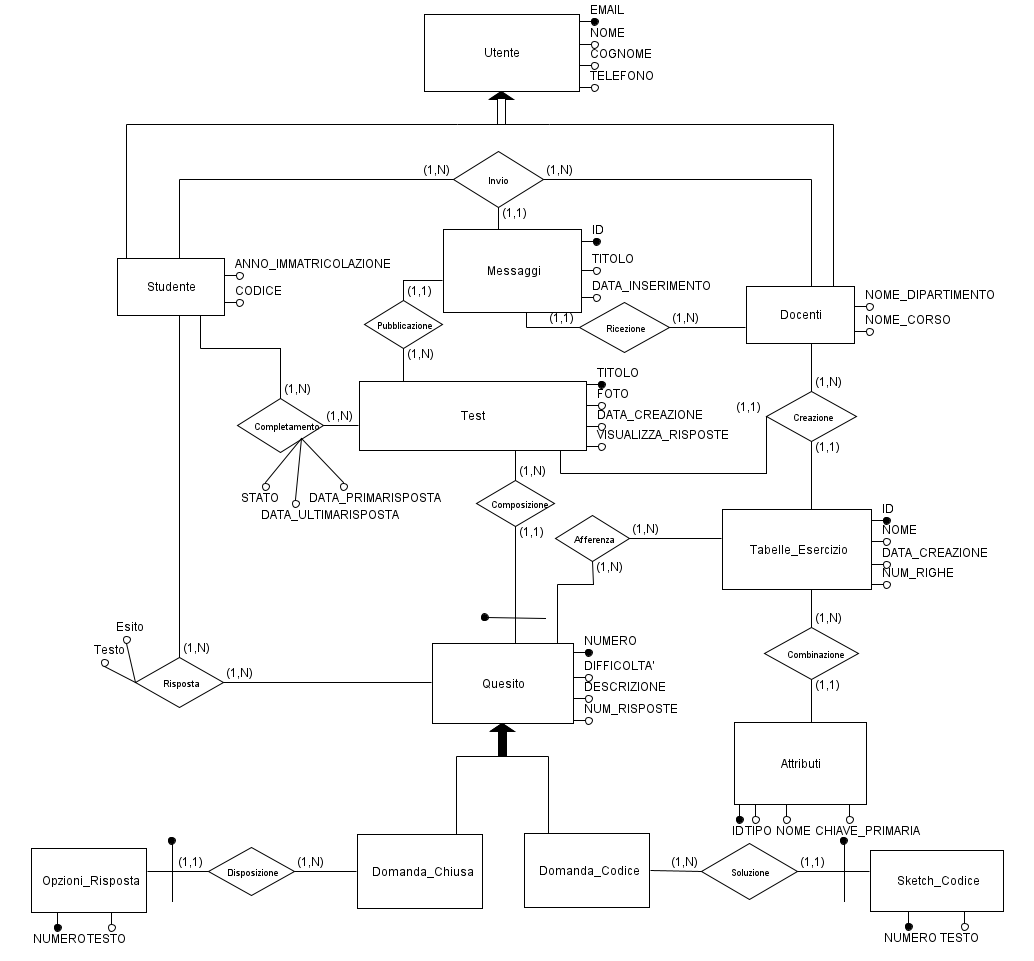
\includegraphics[width=0.7\textwidth]{foto1.png}
    \caption{Modello E-R precedente alla raffinazione.}
\end{figure}

\subsection{Dizionario delle entità}
\begin{table}[H]
    \centering
    \begin{tabular}{|p{3cm}|p{4cm}|p{4cm}|p{3.5cm}|}
        \hline
        \bf Entità & \bf Descrizione & \bf Attributi & \bf Identificatore \\
        \hline
        Utente & Utilizzatore generale dell'applicativo & Email, Password, Nome, Cognome, Telefono & Email \\        
        \hline
        Docente & Docente creatore e ideatore di quesiti e tabelle di esercizio & Nome\_Dipartimento, Nome\_Corso & Email\_Docente \\
        \hline
        Studente & Studente  fruitore della piattaforma per la risoluzione dei quesiti posti & Anno\_Immatricolazione, Codice & Email\_Studente \\
        \hline
        Tabella\_Esercizio & Tabelle contenenti i meta-dati per la realizzazione di eventuali quesiti & ID, Nome, Data\_Creazione, Num\_Righe & ID \\
        \hline
        Attributo & Attributi parte costituente delle tabelle di esercizio, finalizzati per la realizzazione di quesiti & ID, Tipo, Nome, Chiave\_Primaria & ID \\
        \hline
        Test & Test indica l'insieme di quesiti svolti dagli studenti e creati dal docente & Titolo, Foto, Data\_Creazione, Visualizza\_Risposte & Titolo \\
        \hline
        Quesito & Quesito relativo a tematiche svolte durante il corso & ID, Difficoltà, Descrizione, Num\_Risposte & ID, Titolo\_Test \\
        \hline
        Domanda\_Chiusa & Tipologia di quesito, rappresentante una domanda a scelta multipla & . & ID\_Quesito \\
        \hline
        Opzione\_Risposta & Opzioni di risposta relative ad una domanda chiusa & ID, Testo & ID, ID\_Domanda\_Chiusa \\
        \hline
        Domanda\_Codice & Tipologia di quesito, richiedente la formulazione di query SQL & . & ID\_Quesito \\
        \hline
        Skecth\_Codice & Skecth di codice SQL risulutivi rispetto al quesito somministrato & ID, Testo & ID, ID\_Domanda\_Codice \\
        \hline
        Messaggio & Comunicazioni ricevute e inviate tra docenti e studenti & ID, Testo, Titolo, Data\_Inserimento & ID \\
        \hline
        Messaggio\_Studente & Messaggio inviato dallo studente al docente del corso & . & ID\_Messaggio\\
        \hline
    \end{tabular}
    \caption{Descrizione delle entità del modello E-R precedente al raffinamento.}
\end{table}

\subsection{Dizionario delle relazioni}
\large
\begin{table}[H]
    \centering
    \begin{tabularx}{\textwidth}{|X|p{5cm}|p{3cm}|X|}
        \hline
        \bf Relazione & \bf Descrizione & \bf Componenti & \bf Attributi \\
        \hline
        Creazione & Creazione da parte di docenti di tabelle di esercizio e quesiti & Docente, Tabella\_Esercizio, Test & . \\
        \hline
        Completamento & Completamento di un test somministrato da parte degli studenti & Studente, Test & Stato, Data\_UltimaRisposta, Data\_PrimaRisposta \\
        \hline
        Invio & Invio di messaggi da parte di studenti & Studente, Messaggio\_Studente & . \\
        \hline
        Smistamento & Invio e ricezione di comunicazioni dal docente del corso & Docente, Messaggio & . \\
        \hline 
        Pubblicazione & Pubblicazione di comunicazioni afferenti ad uno specifico test & Messaggio, Test & . \\
        \hline
        Ricezione & Ricezione di messaggi emessi da studenti oppure da docenti & Messaggio, Docente & . \\
        \hline
        Risposta & Risposta formulata dagli studenti in relazione ad uno specifico quesito & Studente, Quesito & Esito \\
        \hline
        Composizione & Composizione di un insieme di quesiti rispetto ad un determinato test & Quesito, Test & . \\
        \hline
        Afferenza & Afferenza dei quesiti ideati relativamente a tabelle di esercizio & Quesito, Tabella\_Esercizio & . \\
        \hline
        Combinazione & Combinazione di attributi per la costruzione di tabelle di esercizio & Tabella\_Esercizio, Attributo & . \\
        \hline
        Vincolo Integrità & Vincolo Integrità mantiene tutti i vincoli referenziali tra attributi di tabelle di esercizio & Attributo & . \\
        \hline
        Soluzione & Soluzione alla query SQL richiesta & Domanda\_Codice, Sketch\_Codice & . \\
        \hline
        Disposizione & Disposizione del numero complessivo di opzioni di risposta relative alla domanda sottoposta & Domanda\_Chiusa, Opzione\_Risposta & . \\    
        \hline
    \end{tabularx}
    \caption{Descrizione delle relazioni del modello E-R precedente al raffinamento.}
\end{table}

\subsection{Tavola delle business rules}
\large
\begin{table}[h]
    \centering
    \begin{tabular}[center]{|p{13cm}|}
        \hline
        \bf Regole di vincolo \\
        \hline
        Il campo Codice alfanumerico degli studenti deve avere una lunghezza pari a 16 caratteri \\
        \hline
        Il docente può inserire i vincoli di integrità referenziale tra gli attributi che compongano tabelle di esercizio \\
        \hline
        Il numero progressivo associato ad un quesito è univoco, ma solo all'interno di uno specifico test \\
        \hline
        Il numero delle opzioni di risposta, sia per Domande\_Chiuse che per Domande\_Codice, è univoco, ma solo all'interno dello specifico quesito \\
        \hline
        Uno studente può sottomettere più risposte per lo stesso quesito, ma solo se il test non è in stato Concluso \\ 
        \hline 
        Un messaggio inviato da un docente è recapitato da tutti gli studenti del corso, invece un messaggio comunicato da uno studente è ricevuto dallo specifico docente \\
        \hline
        \bf Regole di derivazione \\ 
        \hline
        Il livello di difficoltà di ogni test consiste in un campo enum, che può assumere esclusivamente tre valori: Basso, Medio oppure Difficile \\
        \hline
        Il campo Num\_Risposte nell'entità Quesito è una ridondanza concettuale \\
        \hline 
        L'attributo Visualizza\_Risposte è un campo booleano, permette di visualizzare o meno le risposte dei quesiti \\
        \hline
        I campi Data\_PrimaRisposta e Data\_UltimaRisposta, della relazione Completamento, devono essere espressi su scala temporale \\
        \hline
        L'attributo della relazione Completamento è un campo enum, il quale può assumere esclusivamente tre valori: Aperto, InCompletamento e Concluso \\
        \hline 
        Il campo Esito della relazione Risposta è un attributo booleano, definisce la correttezza della risposta sottomessa \\
        \hline    
\end{tabular}
    \caption{Descrizione delle regole di vincolo e di derivazione non attuabili tramite il modello concettuale}
\end{table}

\newpage
\section{Progettazione logica}
\large
L'obiettivo di tale sezione promuove la realizzazione del modello logico a partire dalle informazioni del modello E-R. Tuttavia è bene attuare un insieme di possibili passaggi che possano favorire la traduzione, adeguando tematiche di efficienza e correttezza. Pertanto, come da capitolo seguente, è definita la ristrutturazione del entity-relationship diagram, affinchè sia agevolata la traduzione secondo il modello logico, ottimizzando il processo nella sua interezza.

\subsection{Modello E-R raffinato}
\large
\begin{figure}[H]
    \includegraphics*[width=0.75\textwidth]{foto2.png}
    \caption{Modello E-R successivo al raffinamento.}
\end{figure}

\subsection{Analisi delle ridondanze}
\large
In questa sezione sono riportate tutte le considerazioni necessarie per comprendere al meglio l'impatto delle ridondanze sullo schema E-R ideato; con conseguente definizione del costo operazionale sui dati di riferimento. Una fase simile è cruciale per stabilire se determinate informazioni comportano svantaggi significativi, come ad esempio maggiore occupazione di memoria oppure maggiore complessità degli aggiornamenti.\vspace{7pt}\\
Si definiscono le due seguenti nozioni, le quali saranno spesso utilizzate, ossia:
\begin{itemize}[label={-}]
    \itemsep0em
    \item \textit{S$_r$}, lo schema E-R \textbf{con ridondanza}
    \item \textit{S}, \hspace{1px} lo schema E-R \textbf{senza ridondanza}
\end{itemize}
\vspace*{7pt}
Sono specificate un totale di quattro operazioni, relative al campo \textit{Num\_Risposte} dell'entità \textit{Quesito}, le quali si contraddistinguono in: \vspace*{7pt}\\
\hspace*{5pt}\textbf{OP1} \\
\hspace*{5pt}Aggiungere una nuova risposta ad un quesito esistente (10 volte/mese, interattiva) \vspace*{7pt}\\
\hspace*{5pt}\textbf{OP2} \\
\hspace*{5pt}Rimuovere un quesito e tutte le risposte ottenute (2 volte/mese, batch) \vspace*{7pt}\\
\hspace*{5pt}\textbf{OP3} \\
\hspace*{5pt}Visualizzare tutti gli utenti presenti nella piattaforma (1 volte/mese, batch) \vspace*{7pt}\\
\hspace*{5pt}\textbf{OP4} \\
\hspace*{5pt}Contare il numero di risposte per ciascun quesito presente nella piattaforma (2 volte/mese, \hspace*{6pt}interattiva) \vspace*{7pt}\\
Consecutivamente si calcolano i costi operazionali dello schema E-R con ridondanza, esplicitando tutti gli elementi necessari, suddivisi in:
\begin{itemize}[label={ }]
    \itemsep0em 
    \item {\small\textbf{TAVOLA ACCESSI.} \\ 1 per RISPOSTA, 1 per QUESITO, 1 per DOMANDA\_CHIUSA, 1 per DOMANDA\_CODICE} \vspace*{2pt}\\ C(OP1) = 10 * 1 * (2 * 4 + 0) = 80 \vspace*{2pt} 
    \item {\small\textbf{TAVOLA ACCESSI.} \\ 10 per RISPOSTA, 1 per QUESITO, 1 per DOMANDA\_CHIUSA, 1 per DOMANDA\_CODICE} \vspace*{2pt}\\ C(OP2) = 2 * 0.5 * (2 * 13 + 0) = 26 \vspace*{2pt}
    \item {\small\textbf{TAVOLA ACCESSI.} \\ 50 per UTENTE, 50 per STUDENTE, 50 per DOCENTI} \vspace*{2pt}\\ C(OP3) = 1 * 0.5 * (0 + 150) = 75
    \item {\small\textbf{TAVOLA ACCESSI.} \\ 20 per QUESITO, 20 per DOMANDA\_CHIUSA, 20 DOMANDA\_CODICE } \vspace*{1pt}\\ C(OP4) = 2 * 1 * (0 + 60) = 120
\end{itemize}
\hspace*{15pt}C(S$_r$) = 80 + 26 + 75 + 120 = 301 \vspace*{7pt}\\
Si calcolano i costi operazionali dello schema E-R senza ridondanza, suddivisi in:
\begin{itemize}[label={ }]
    \itemsep0em 
    \item {\small\textbf{TAVOLA ACCESSI.} \\ 1 per RISPOSTA} \vspace*{2pt}\\ C(OP1) = 10 * 1 * (2 * 1 + 0) = 20 \vspace*{2pt} 
    \item {\small\textbf{TAVOLA ACCESSI.} \\ 10 per RISPOSTA, 1 per QUESITO, 1 per DOMANDA\_CHIUSA, 1 per DOMANDA\_CODICE} \vspace*{2pt}\\ C(OP2) = 2 * 0.5 * (2 * 13 + 0) = 26 \vspace*{2pt}
    \item {\small\textbf{TAVOLA ACCESSI.} \\ 50 per UTENTE, 50 per STUDENTE, 50 per DOCENTI} \vspace*{2pt}\\ C(OP3) = 1 * 0.5 * (0 + 150) = 75
    \item {\small\textbf{TAVOLA ACCESSI.} \\ 200 per RISPOSTA, 20 per QUESITO, 20 per DOMANDA\_CHIUSA, 20 per DOMANDA\_CODICE} \vspace*{2pt}\\ C(OP4) = 2 * 1 * (0 + 260) = 520
\end{itemize}
\hspace*{15pt}C(S) = 20 + 26 + 75 + 520 = 641 \vspace*{7pt} \vspace*{7pt}\\
Si osserva ora l'occupazione di memoria di entrambi i diagrammi, in cui si manifesta:
\begin{itemize}[label={-}]
    \itemsep0em
    \item M(S$_r$) = X + 20 * 4 = X + 80 byte
    \item M(S) = \hspace*{1pt}X byte
\end{itemize}
Terminate tutte le operazioni riferite all'analisi delle ridondanze, si osserva come il mantenimento comporti a vantaggi significativi, piuttosto che l'eliminazione. Infatti il rapporto della metrica $C(S) \div C(S_r)$ restituisce un valore che si aggira attorno a 2, in questo caso è conveniente mantenere l'attributo Num\_Risposte, dettata anche dall'irrisorio overhead introdotto, pari a 80 byte.

\subsection{Lista delle tabelle con i vincoli di chiave}
\large
Dopo aver svolto le fasi principali che agevolano il processo di traduzione, nella sezione consecutiva si osserva la descrizione del modello logico di riferimento, il quale fornisce l'insieme di tabelle che caratterizzano il database e i differenti attributi relativi ad ogni specifica relazione. Si evidenzia la presenza delle chiavi primarie, segnalate attraverso una sottolineatura delle colonne che compongano il vincolo.\vspace*{7pt}
\begin{itemize}[label={ }, leftmargin=*, wide=1pt]
    \itemsep0em
    \item Utente(\underline{Email}, Pswd, Nome, Cognome, Telefono)
    \item Studente(\underline{Email\_Studente}, Codice, Anno\_Immatricolazione)
    \item Docente(\underline{Email\_Docente}, Nome\_Diparitmento, Nome\_Corso)
    \item Tabella\_Esercizio(\underline{ID}, Nome, Data\_Creazione, Num\_Righe)
    \item Attributo(\underline{ID}, ID\_Tabella, Tipo, Nome, Chiave\_Primaria)
    \item Vincolo\_integrita(\underline{Referente}, \underline{Referenza})
    \item Test(\underline{Titolo}, Email\_Docente, Foto, Data\_Creazione, Visualizza\_Risposta)
    \item Quesito(\underline{ID}, \underline{Titolo\_Test}, Difficolta, Descrizione, Num\_Risposte)
    \item Afferenza(\underline{ID\_Quesito}, \underline{ID\_Tabella}, \underline{Titolo\_Test})
    \item Domanda\_Chiusa(\underline{ID\_Domanda\_Chiusa})
    \item Opzione\_Risposta(\underline{ID}, \underline{ID\_Domanda\_Chiusa}, Testo)
    \item Domanda\_Codice(\underline{ID\_Domanda\_Codice})
    \item Skecth\_Codice(\underline{ID}, \underline{ID\_Domanda\_Codice}, Testo)
    \item Completamento(\underline{Titolo\_Test}, \underline{Email\_Studente}, Stato, Data\_UltimaRisposta, Data\_PrimaRisposta)
    \item Risposta(\underline{Email\_Studente}, \underline{ID\_Quesito}, Testo, Esito)
    \item Messaggio(\underline{ID}, Email\_Docente, Titolo, Testo, Data\_Inserimento, Titolo\_Test)
    \item Messaggio\_Studente(\underline{ID\_Messaggio\_Studente}, Email\_Studente)
\end{itemize}

\subsection{Lista dei vincoli inter-relazionali}
\large
Quest'ultima parte del capitolo, riporta in maniera esplicita tutti i vincoli inter-relazionali che intercorrono tra le differenti tabelle, disposti nello stesso ordine in cui sono visualizzate le relazioni nel paragrafo precedente.
\begin{itemize}[label={ }, leftmargin=*, wide=1pt]
    \itemsep0em
    \item Studente.Email\_Studente \textbf{-->} Utente.Email
    \item Docente.Email\_Docente \textbf{-->} Utente.Email
    \item Attributo.ID\_Tabella \textbf{-->} Tabella\_Esercizio.ID
    \item Vincolo\_Integrità.Referente \textbf{-->} Attributo.ID
    \item Vincolo\_Integrità.Referenziato \textbf{-->} Attributo.ID
    \item Test.Email\_Docente \textbf{-->} Docente.Email\_Docente
    \item Quesito.Titolo\_Test \textbf{-->} Test.Titolo
    \item Afferenza.ID\_Quesito \textbf{-->} Quesito.ID
    \item Afferenza.ID\_Tabella \textbf{-->} Tabella.ID
    \item Afferenza.Titolo\_Test \textbf{-->} Test.Titolo
    \item Domanda\_Chiusa.ID\_Domanda\_Chiusa \textbf{-->} Quesito.ID
    \item Opzione\_Risposta.ID\_Domanda\_Chiusa \textbf{-->} Domanda\_Chiusa.ID\_Domanda\_Chiusa 
    \item Domanda\_Codice.ID\_Domanda\_Codice \textbf{-->} Quesito.ID
    \item Skecth\_Codice.ID\_Domanda\_Codice \textbf{-->} Domanda\_Codice.ID\_Domanda\_Codice
    \item Completamento.Titolo\_Test \textbf{-->} Test.Titolo
    \item Completamento.Email\_Studente \textbf{-->} Studente.Email\_Studente
    \item Risposta.Email\_Studente \textbf{-->} Studente.Email\_Studente
    \item Risposta.ID\_Quesito \textbf{-->} Quesito.ID
    \item Messaggio.Email\_Docente \textbf{-->} Docente.Email\_Docente
    \item Messaggio.Titolo\_Test \textbf{-->} Test.Titolo
    \item Messaggio\_Studente.ID\_Messaggio\_Studente \textbf{-->} Messaggio.ID
    \item Messaggio\_Studente.Titolo\_Test \textbf{-->} Studente.Email\_Studente
\end{itemize}


\newpage
\section{Normalizzazione}
\large
\dots

\section{Riflessioni}
\large
\dots

\subsection{Sviluppo alternativo}
\large
\dots

\section{SQL}
\large 
\dots

\end{document}